\newcommand{\st}{ \ | \ }

\section{Requirements for New Graph Syntax}
	\label{s:requirements}
	The ultimate goal of the new graph--based syntax presented here is to be able to 
	fully describe the general structure of an MDAO problem independently of any solution information, 
	while still being able to accomodate the more specific case when a solution 
	strategy is applied. In order to achieve that goal 
	the graph needs to accomodate a number of constructs of MDAO problems: 
	\begin{itemize}
		\item Analysis tools and connections between them
		\item Design variables, objectives, and constraints
		\item Local and global properties
		\item Coupling between analyses
		\item Multi-fidelity analyses
	\end{itemize}

	Beyond those basic constructs, there are also three phases of a design process that 
	all need to be representable with the new syntax. Firstly there is the initial problem definition
	phase where the specific analysis tools and design goals are identified. At the end of this phase, 
	a single formal problem formulation is selected specifying design variables, constraints, objectives, 
	analysis tools, etc. Lastly some specific procedure for solving the problem is selected, for example 
	picking an MDAO optimization architecture. Using the proposed graph syntax, each of these phases 
	can be represented with the following three graphs:
	\begin{itemize}
		\item Maximal Connectivity Graph (MCG)
		\item Fundamental Problem Graph (FPG)
		\item Problem Solution Graph (SPG)
	\end{itemize}

	The \emph{maximal connectivity graph} represents the first phase with all 
	analysis codes being considered and all possible connections between them also present. The second graph 
	is the \emph{fundamental problem graph}, which is the smallest possible graph 
	that still fully defines a given problem formulation. Finally, a \emph{specific problem formulation} 
	may be represented by including additional edges and nodes to represent the 
	solution strategy being employed to solve the problem. 

	The relationship between these three graphs is depicted in Figs.~\ref{f:tree} and \ref{f:hourglass}. 
	The tree diagram demonstrates the fact that it is generally possible to obtain 
	multiple FPGs from a single maximal connectivity graph. This  may correspond to 
	different down--selections of analysis codes, different connections between them, 
	or both. Each down--selection shrinks the number of possible FPGs that could be reached 
	until only one is remaining. Then, from a single FPG, different PSGs may be obtained by implementing 
	different solution strategies. If you consider the size of a graph to be the sum of all of its
	edges and nodes then the hourglass shape in Fig. \ref{f:hourglass} illustrates how
	the MCG gets reduced to a single FPG, then multiple possible PSGs exist to solve the problem.
	In other words the FPG is obtained from the MCG by removing nodes and edges, 
	and the PSG is obtained from the FPG by adding nodes and edges.

	\begin{figure}[htb!]
		\centering
		\subfigure[number of possible graphs]{
		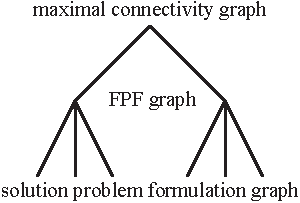
\includegraphics[width=2.0in]{images/tree}
		\label{f:tree}
		}
		\subfigure[graph size]{
		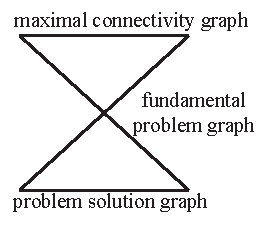
\includegraphics[width=2.0in]{images/hourglass}
		\label{f:hourglass}
		}
	\caption{The relationship between the MCG, FPG, and PSG.}
	\end{figure}

\section{Syntax Definition}
	\label{s:syntax definition}
	In this section we present the necessary graph theory fundamentals to 
	construct the graphs discussed above. 
	The notation used in this work is adapted from Diestel \cite{Diestel2010}. 
	A \emph{graph} is a pair $G = (V,E)$ of sets such that $E \subseteq V \times V$, 
	which means that the elements of $E$ are 2--element subsets of $V$. The set $V$ 
	contains the \emph{vertices} or \emph{nodes} and the set $E$ contains the \emph{edges}.
	For a \emph{directed graph*} (or \emph{digraph}) we construct $E$ as a set of ordered pairs instead 
	of a set of sets. Each ordered pair represents an edge starting at the node 
	indicated by the first entry and directed to the node indicated by the second 
	entry. Edge $e$ = $(x,y)$ may be referred to simply as $xy$. For node $v \in V$ 
	the edges directed out are given by $E(v)$ and the edges directed into $v$ are given 
	by $E^{-1}(v)$; $E(E(v))$ is denoted as $E^2(v)$, and likewise for additional levels. 
	If $E$ is not a one--to--one mapping, $E(v)$ may be the empty set, a single node, or a set of nodes.
	\begin{figure}[htb!]
		\begin{center}
		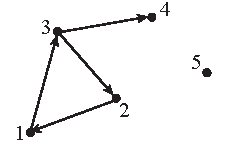
\includegraphics[width=1.5in]{images/example_directed_graph}
		\end{center}
		\vspace{-20pt}
	\caption{Example directed graph.}
	\label{f:example directed graph}
	\end{figure}
	As an example, for the directed graph shown in Fig.~\ref{f:example directed graph} we have
	\begin{IEEEeqnarray*}{rCl}
	V & = & \{1,2,3,4,5\}, \\
	E & = & \big\{(1,2),(3,2),(1,3),(3,4)\big\}.
	\end{IEEEeqnarray*}

	%does this belong in the analysis block section???? 
	Let $I$ be a nonempty set of counting numbers such that for each $i \in I$ there is a corresponding set $A_i$. 
	The set of sets $\mathcal A = \{A_i \st i \in I\}$ is called an indexed family of sets with index $i$ and 
	indexing set $I$\cite{smith2006}. 
	The union over this family of sets can be described in a few different ways:
	\begin{equation}
	\bigcup_{i \in I} A_i = \bigcup_{A \in \mathcal A} A = \{x \st x \in A \txt{ for some } A \in \mathcal A\}.
	\end{equation}

	Lastly, the cardinality of a set $B$ is the number of elements in $B$ and is denoted as $|B|$.

\subsection{Node and Edge Types}
	\label{ss:types}
	We now define different types of nodes and edges with specific properties to compose graphs used to represent an MDAO problem. 
	There are three node types:  
	\begin{description}
	\item[variable: ] represents scalar or array data
	\item[model:] responsible for mapping inputs to outputs
	\item[driver:] control logic capable of managing iteration
	\end{description}

	In addition to the three node types, there are two edge types: 

	\begin{description}
	\item[connection edge:] Exchange of information between two nodes. These edges 
	can either be fixed (can not be removed from graph) or free (can be removed). 
	\item [implicit edge:] Implicit passing of information from a driver node to a 
	  variable node. A single variable node can have many incomming implicit edges. These edges are 
	  free and can be added or removed from the graph. 
	\end{description}

	[[Insert legend for node and edge types]]

	In Alexandrov and Lewis's REMS syntax only two node types were present, variable 
	and function, and only one edge type\cite{alexandrov2004}. We've chosen to rename the ``function'' node 
	type to ``model'' to be more consistent with modern MDAO frameworks. The present work 
	adds two more node types and one more edge type to the syntax to allow descriptive
	graphs for all three phases of the design process. 

\subsection{Rules for Nodes and Edges}
	\label{ss:rules}
	There are specific rules for the usage of these nodes and edges.
	The driver node and the implicit edge are only allowed to be present in PSGs. All 
	other node and edge types can be present in any of the three graphs, subject to these restrictions: 
	\begin{enumerate}
	\item A model node can only have one edge directed to or from another model node.
	\item A model node can only have fixed connection edges directed in or out.
	\item A model node must have at least one edge directed in and at least one edge 
	  directed out.
	\item If a variable node has an outgoing edge to a model node then it may not have 
	  any other outgoing edges.
	\end{enumerate}

\subsection{In-degree and Out-degree}
	\label{s:indegree-outdegree}
	The \emph{in--degree} of a node is the number of connection edges directed in and 
	is denoted as $\txt{deg}^-(v)$, and the \emph{out--degree} 
	is the number of connection edges directed out and it is denoted as $\txt{deg}^+(v)$.
	The degree of a given node is only a function of the connection edges 
	attached to it. The number of implicit edges is not relevant since any number 
	of drivers could be involved, at different parts of an solution process. For 
	example in a sequential optimization where a global optimizer is first applied
	and a gradient based one is applied second, design variables would have incomming 
	implicit edges from both optimizers but this would not affect the in--degree of those
	variable nodes. 
	((DP:I started to remove any reference to the edge type in these definitions but then saw that you needed it. The reason I did that was because in--degree and out--degree are basic graph theory terms. What if the reference to implicit edges is handled with the upper in--degree limit, i.e. after the FPG is obtained the upper indegree limit for the design variable nodes is relaxed (increased) so that it isn't a problem what is or isn't counted?))

	((DP:the definitions were in/out degree were not in my book, I had to get them from wikipedia, where they are spelled indegree and outdegree))

	We also define the \emph{upper in--degree limit} 

	\begin{equation}
	\txt{deg}_u^-(v):V \to \mathbb{N}
	\end{equation} 
	and the \emph{lower in--degree limit} as
	\begin{equation}
	\txt{deg}_l^-(v):V \to \mathbb{N}.
	\end{equation}
	These user-specified limits govern the number of connection edges that may be directed into a variable
	node for a valid graph. Consider a variable node $v$ with
	$\txt{deg}_u^-(v) = \txt{deg}_l^-(v) = 1$. In this case, $v$ must have exactly one
	incomming explicit edge or the graph is invalid. Two possiblities exist for voilating 
	these limit conditions: 
	\begin{description}
	  \item[hole: ] The number of incomming edges is less than the lower indegree limit:
		\begin{equation} \txt{deg}^-(v) < \txt{deg}_l^-(v) \label{e:hole} \end{equation}
		This represents a lack of information being supplied to the node.

  \item[collision: ] The number of incomming edges is greater than $ \txt{deg}_u^-(v)$. 
    \begin{equation} \txt{deg}^-(v) > \txt{deg}_u^-(v) \end{equation}
\end{description} 
These violations will be managed in order to seek a working problem formulation.

\section{Graph Representation of MDAO Constructs}
\label{s:graph representation}
In this section we will make use of the Sellar problem, described in 
Eqn. \ref{eqn:simple_fpf}. The graph representation of the Sellar problem, 
using the new stynax, is presented in Fig. \ref{f:sellar_graph_full}. Throughout
the rest of this section, different sub-graphs or slight modifications of 
the full graph will be used to demonstrate the important MDAO constructs within
this graph syntax.

\begin{figure}[htb!]
    \begin{center}
    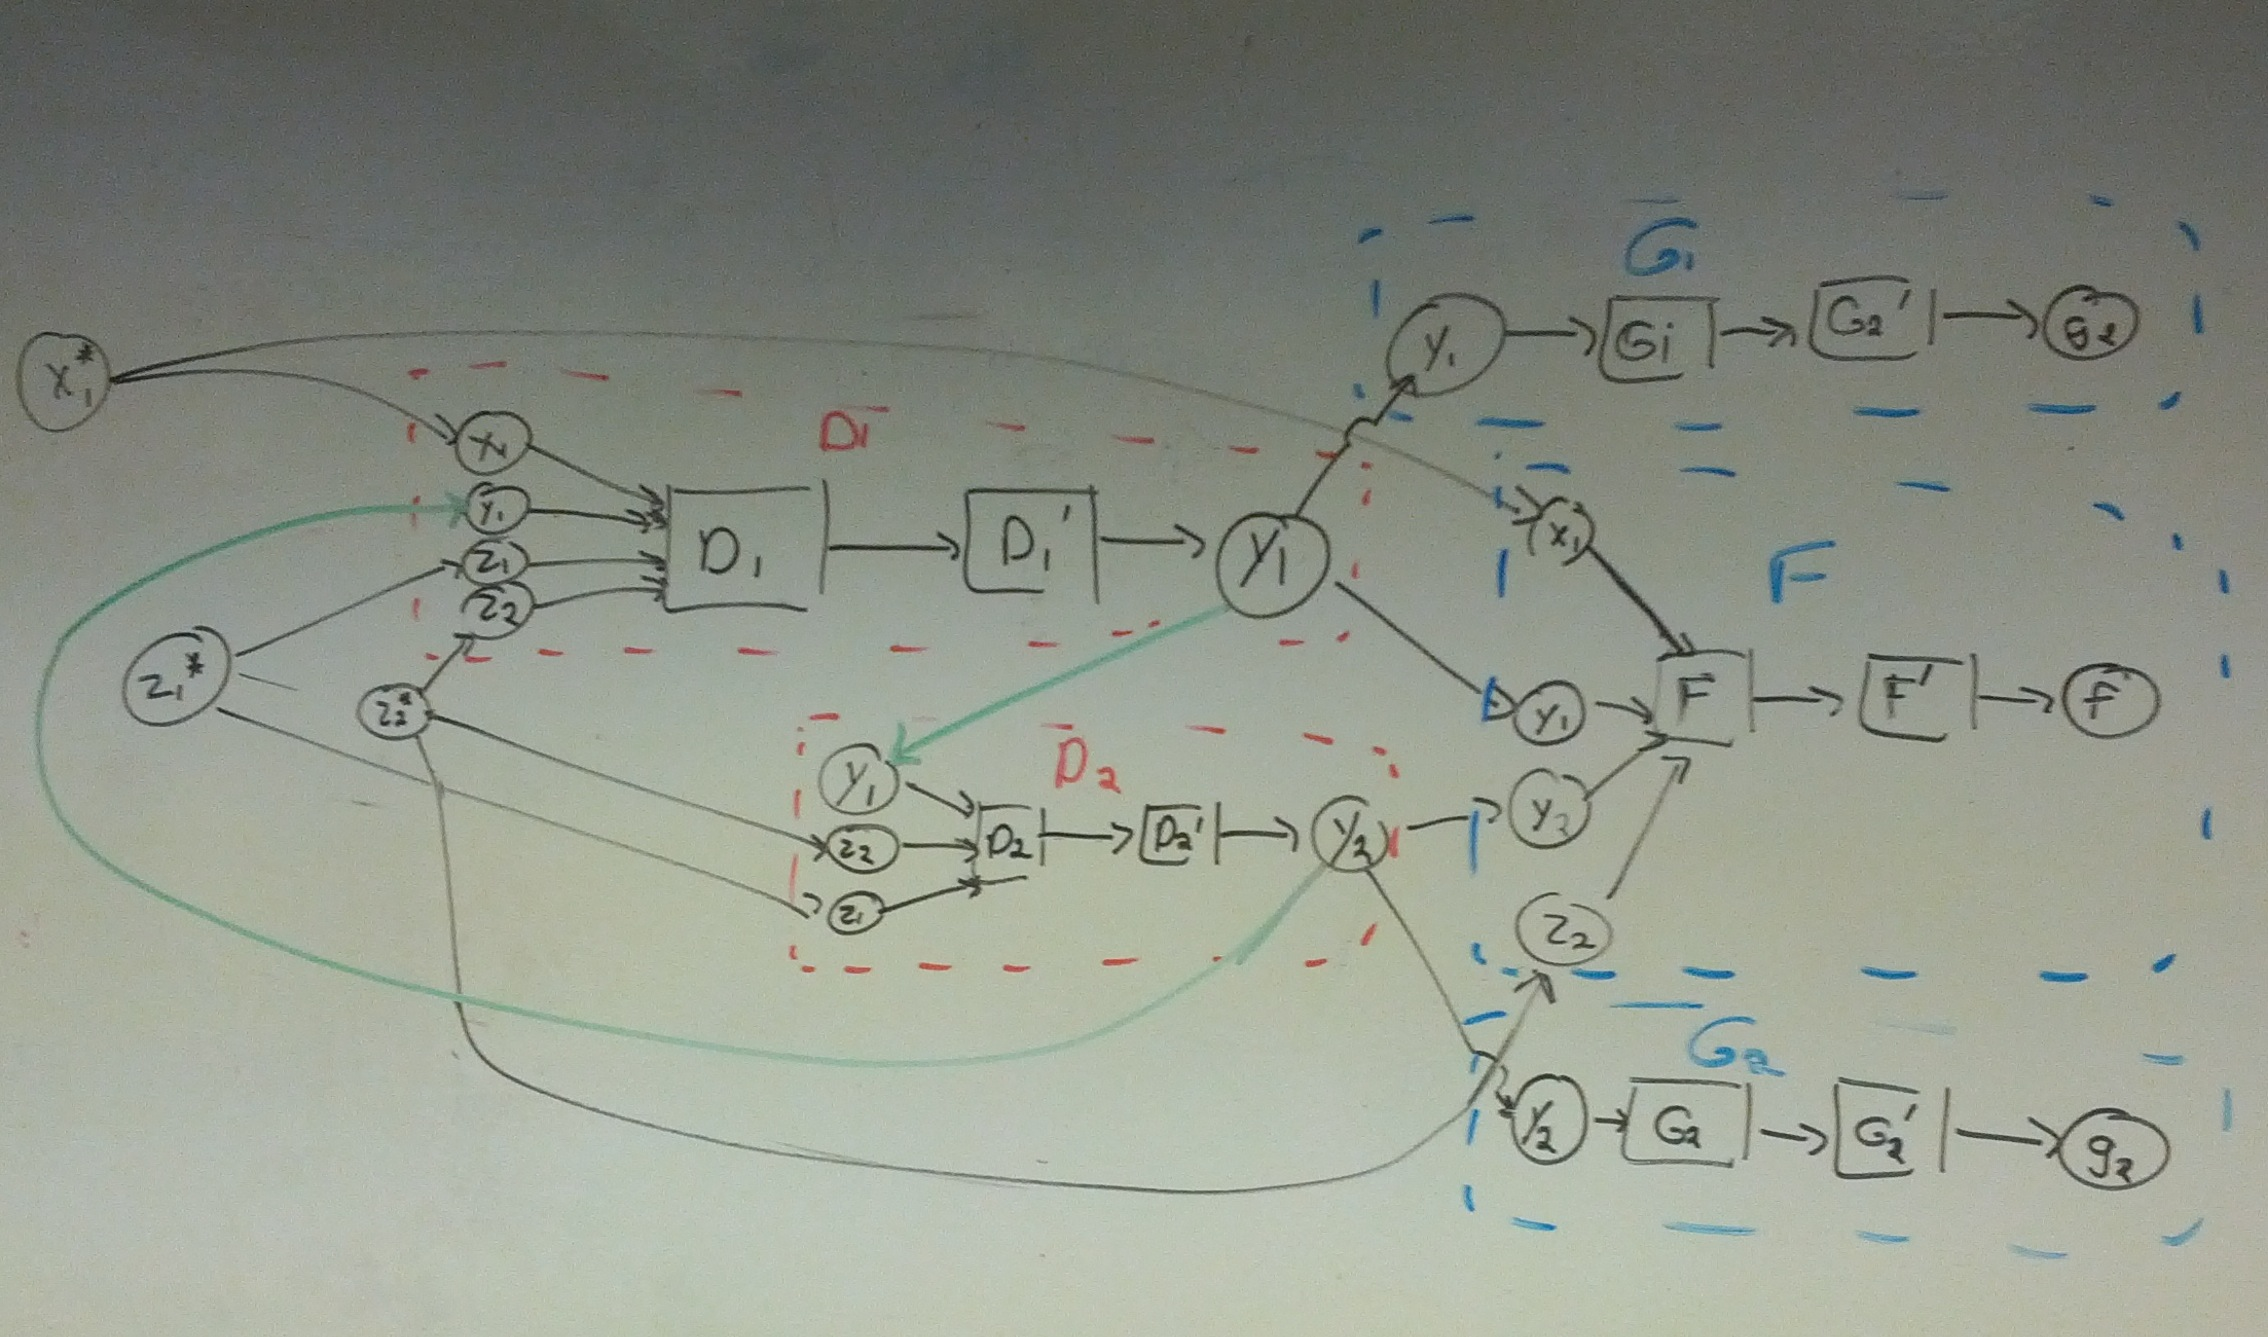
\includegraphics[width=4in]{images/sellar_graph_full}
    \end{center}
    \vspace{-10pt}
\caption{Graph of the Sellar problem formulation}
\label{f:sellar_graph_full}
\end{figure}

%As discussed in Sec.((intro)), the digraph must be able to describe the individual aspects of an MDAO problem.
\subsection{Analysis Blocks and Connections}
\label{ss:analysis blocks and connections}
Analysis tools take in a number input variables and then perform some work to calculate 
the values for their respective outputs. In an MDAO graph, this process is 
represented by a group of nodes and edges called an \emph{analysis block}, 
shown in Fig. \ref{f:analysis block}. Within an analysis block each variable 
node represents a single input or output and is connected 
to a single model node via a fixed edge. Note that in Fig. \ref{f:analysis block}, 
the analysis block contains two model nodes, with a single edge connecting them. 
This edge represents the necessary calculations to map given inputs 
to proper output values. If constructing a weighted graph, the weight calculation edge 
provides the opportunity to computational cost. However, it is also allowed to skip 
this edge and have both incomming and outgoing edges to variables through a single model 
node for a given analysis block. Although analysis blocks are comprised of multiple nodes and edges, since all 
the edges within them are fixed, they become fixed sub-graphs within a graph.

\begin{figure}[htb!]
    \begin{center}
    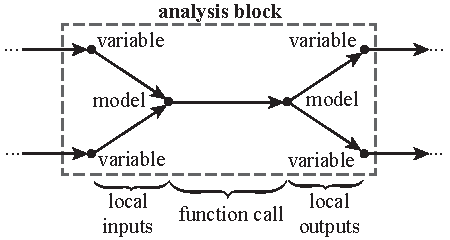
\includegraphics[width=4in]{images/analysis_block}
    \end{center}
    \vspace{-10pt}
\caption{Example analysis block. The each node type and edge type is labeled in italics and annotated parenthetically.}
\label{f:analysis block}
\end{figure}

	Variable nodes in an analysis block can be distinguished as either an input or an output by the manner in which they are connected. As shown in Fig.~\ref{f:analysis block}, inputs are any variable nodes that have an outgoing edge into a model 
	node. Conversely, outputs are any variable nodes that have an incoming edge from a model node. 
	Note that by this definition, inputs and outputs can only exist when variable nodes poses an 
	edge joining them to a model node. 
	((DP:I'm not sure what the sentences before or after this comment mean))
	These are labeled out as 
	local inputs and local outputs. The variables are local because they are explicitely tied
	to the analysis block and have no relevance without it. 

MDAO problems require that information be passed between sets of analyses. When 
information from the output of one analysis block is passed, or connected, to the 
input of another analysis block, a new connection edge is added connecting the two 
variable nodes involved in the exchange. These connection edges are free, unlike the edges 
within an analysis block, they could be added or removed depending on the needs
of a given design problem. In other words, free connection edges are created by 
engineers linking the output of one tool to the input of another one. Note that 
it is allowed for a single output to have outgoing connection edges to multiple 
downstream inputs. 

\subsection{Design Variables}
((DP:I'm thinking we might also need the upper indegree limit to be zero as well, because setting only the lower indegree limit makes the node a design variable if it didn't have any incoming edges. It's seems possible that in the MCG a node has incoming edges but the user wants it to be a design variable. I can make the change if you agree.))
For the Sellar problem, there are three design variables, $x_1^*$, $z_1^*$, and $z_2^*$. In Fig. 
\ref{f:sellar_graph_full}, these are the only three holes (nodes without out 
incomming edges) in the graph. 

\begin{figure}[htb!]
  \begin{center}
  [NOTE: Re-work this one to match $D_2$ from Sellar]
    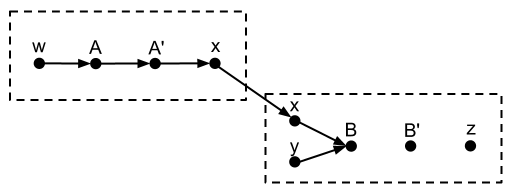
\includegraphics[width=.6\textwidth]{images/design_vars_graph}
  \end{center}
  \caption{Notional graph with two potential design variables \label{f:designvars}}
\end{figure}

More formally stated, given a MCG with the $\txt{deg}_l^-(v)=1$ for all nodes, 
there will likely be a set of holes preventing a valid FPG from being obtained. 
Each hole represents a node that could potentially become a design variable. 
It is up to the designer to examine each and decide if it is appropriate to 
consider it a design variable, in which case the designer shall set the lower 
indegree limit to be zero. However, some variable holes may not actually be 
suitable as a design variable. For instance, if an aircraft mission analysis 
code requires a drag input which ends up being a hole then it's likely best to 
leave$\txt{deg}_l^-(v)=1$ and find a new analysis code to fill the hole in graph. 

So a design variable is defined as any variable node with $\txt{deg}_l^-(v)=0$. 
This, by definition, means that design variables are not holes in the graph, since 
they have not violated their lower in-degree limit. Regardless, 
when working with a MCG or FPG, only connection edges are allowed, so a design 
variable in either graph will be a variable with no incomming edges edges. For a valid PSG 
any design variable node would have at least one, but possibly multiple, incomming 
implicit edges from one or more driver nodes. 

\subsection{Objectives, and Constraints}
\label{ss:objectives and constraints}
Like design variables, objectives and constraints are also constructs that need 
to be identified when setting up a given design problem. In the case of 
objective functions single output values could be selected, but commonly multiple 
values are assembeled together via simple algebraic expressions to form a composite 
objective function. (e.g. The objective function from Eqn. \ref{eqn:simple_fpf} is
$x_1^2+z_2+y_1+e^{-y_2}$). Constraints are always given in the 
form of either an inequality or an equality. (e.g. a constraint from Eqn. 
\ref{eqn:simple_fpf} is $\frac{y_1}{3.16}-1\geq0$.) By convention, 
constraints are usually given such that some expression will be less than or equal 
to zero, so any positive value would violate the constraint. For both objective 
and constraints, these simple expressions take some inputs and map them to an
output value of significance to the overall design problem. 

These operations, though very simple, are effectively the same kind of task 
performed by an analysis block. A constraint or objective function can therfore 
be represented as another analysis block on the graph, with it's own input and 
output variable nodes. Although fundamentally no different than an analysis block, 
for clarity and convience it is useful to distinguish between regular analysis 
blocks and those that arise from the addition of objectives or constraints to 
the graph. So we define an expression block, as the collection of variable and model 
nodes related to a given objective or constraint function. Fig. \ref{f:obj-cons}
shows a notional problem graph augmented with expression blocks and appropriate 
connection edges. 


\begin{figure}[htb!]
  \begin{center}
    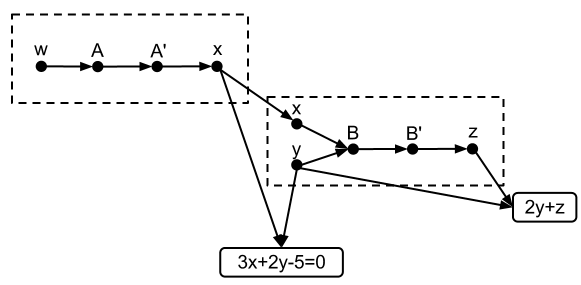
\includegraphics[width=.6\textwidth]{images/obj_const_graph}
  \end{center}
  \caption{Notional graph with and objective and constraint nodes \label{f:obj-cons}}
\end{figure}


\subsection{Local vs Global Nodes}

  A simple definition of a global node is any node that involves information 
  from more than one analysis block. Likewise, a local node is any node 
  that involves information from only a single analysis block. As stated before, variable 
  nodes with fixed edges directed to model nodes (as part of an analysis block) are inherently local 
  and similarly model nodes are also local. Global variables are a part of many 
  MDAO problems and must be representable in the graph. Follwoing our simple definition
  any variable node that had multiple incomming or outgoing edges, would be global. 
  In Fig. \ref{f:sellar_graph_full} the variable nodes for $x_1^*$, $z_1^*$, and $z_2^*$ 
  have multiple outgoing edges and would be considered global. 

  Note that the variable $x_1$ from the Sellar problem is usually refered to as 
  a local variable, which is contradicted by the given graph. This discrepancy 
  arises from the explicit treatment of objectives and constraints as separate 
  expression blocks. Normally in the Sellar problem $x_1$ is considered a local 
  variable because it only directly affects analysis block $D_1$. By forcing
  the expansion of $F$ into an expression block with its own inputs, then $F$ 
  gets it's own copy of the $x_1$ variable. This necessitates the creation 
  of the global $x_1^*$ node in the graph with two outgoing edges to link the 
  two $x_1$ inputs nodes in the different blocks. Interestingly, using this 
  definition, where $x_1^*$ is a global variable fits nicely within 
  the structure of Braun's Colaborative Optimization (CO) archtiecture \cite{braun_thesis}. 
  The rules of setting up a problem with CO require that each discipline be 
  given an independent local copy of all global variables, while any local 
  variables are retained uniquely within their respective disciplines. But 
  when a local design variable shows up explicitely in the objective function 
  or global constraint then a global variable is created, and the discipline again 
  gets an independent local copy of it. Given our definition of global vs local
  variable nodes, no such exception for local variables is necessary. When you 
  include a given variable in an expression node, it becomes global by definition 
  and should be treated as such in CO. 

  Analysis and expression blocks can also have a locality defined for the set of 
  nodes and edges within the block. Their locality is determined by the 
  incomming and outgoing edges from the block as a whole. Fig. \ref{f:sellar_graph_full} has expression blocks for each constraint, $G_1$ and $G_2$. Both constraints are 
  local to their respective analysis blocks. But the expression block for $F$ 
  has incomming edges from $D_1$ and $D_2$, so it would considered global. 

  \begin{figure}
      \begin{center}
      %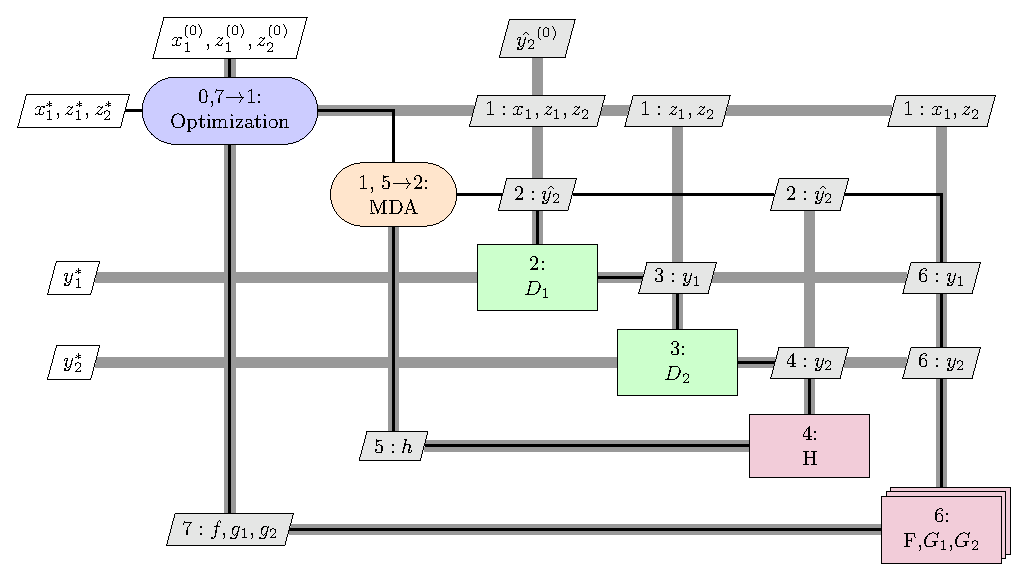
\includegraphics[height=.25\textheight]{XDSM/simple}
      [[insert graph here]]
      \caption{A simple graph with local and global nodes \label{f:local_global}}
      \end{center}
  \end{figure}

  Simply stating that any node or block with incomming or outgoing edges
  from more than one other node or block is global works glosses over a more 
  subtle aspect of some MDAO problems. The locality of any node in a graph is 
  a relative property. For instance, a single node might have outgoing edges 
  to two separate analysis blocks, $A$ and $B$, but none to a third, $C$. Then 
  you could say that this node was global with respect to $A$ and $B$, but local 
  to the group $A,B$ with respect to $C$. This situation produces a natural 
  hierarchy in a graph, where you can form increasingly smaller groups as you 
  segment problem into finer localities. When solving a problem using 
  a heirarchical decomposition approach, there are various techniques for 
  partitioning that are effective in different scenarios 
  \cite{krishnamachari1997optimal,Perez2004,sobieszczanski1997,allison2009optimal,michelena1997hypergraph}. 

\subsection{Coupling Between Analyses}

  Coupling exists in a design problem when a set of two or more analyses each depend on the
  others outputs. Consider the notional problem from section \ref{sec:spg_vs_fpg} where two 
  analyses, $A$ and $B$ are coupled through their respective variables. The graph of this 
  is shown in Fig. \ref{f:coupling}. In the graph $A.z$ has an outgoing connection 
  edge to $B.z$, indicating that there is a connection between the two. 
  Similarly a connection exists between $B.y$ and $A.y$. These two connections form 
  a cycle which represent the coupling between them. This cycle means that blocks $A$ and $B$ need
  to be iterated on untill they converge. 

  \begin{figure}
      \begin{center}
      %\includegraphics[height=.25\textheight]{}
      [INSERT GRAPH HERE]
      \caption{Graph of a notional problem with simple coupling \label{f:coupling}}
      \end{center}
  \end{figure}

	It is important to note that the cycle in graph in Fig.~\ref{f:coupling} does not contain 
	any driver nodes. That means that no solver, optimizer, or other iterative construct is 
	invovled in the coupling. This absence is intentional, as the coupling is an inherent part 
	of the problem. This corresponds directly to Eqn.~\ref{eqn:simple_fpf}, where 
	each equality constraint is one edge in the graph. Transitioning to either 
	Eqn.~\ref{eqn:simple} or Eqn.~\ref{eqn:simple2} means selecting one of the nodes as the starting point 
	for the iteration and indicating which associated analysis block should be executed first. 

	Larger problems can contain more complex cycles in their FPG, indicating more 
	complex coupling between analyses. A cycle can contain more than 
	just two analysis blocks. Multiple independent cycles can exist, indicating 
	independent coupling relationships. Cycles can also overlap, where the same analysis 
	blocks are involved in multiple different coupling cycles. All of these situations
	arise naturally as the size of problems grows, and managing this coupling may
	become difficult. From the perspective of the graph, the problem reduces down to 
	an ordering challenge. For each cycle in the graph, an analysis block needs to be selected 
	to start the iteration from. Rogers' DEMAID tool uses a genetic algorithm to find an ordering 
	that minimizes the overall coupling of the system by separating independent 
	cycles in the graph \cite{rogers1996,rogers1996demaid}. In the present work, Sec.~\ref{s:example problem}.\ref{ss:obtaining an FPG} will suggest that an FPG may be obtained with respect to the number of cycles or the length of these cycles, etc.

\subsection{Multi--fidelity Problems}
	\label{ss:multi-fideliy problems}
	A multi--fidelity problem can be characterized by two or more different analyses 
	each calculating the same data. Mapping this type of multi--fidelity situation 
	onto a graph will yield two analysis blocks, each with their own output 
	variable nodes, having outgoing edges to a third analysis block that needs the 
	data as input. Figure \ref{f:collision-example} shows a notional problem 
	that exhibits this structure, where the key feature is that variable node $y$ in 
	analysis block $C$ has two incoming edges. 
	\begin{figure}
	  \begin{center}
	  %\includegraphics[height=.25\textheight]{}
	  [INSERT GRAPH HERE]
	  \caption{Graph of a notional multi-fidelity problem \label{f:collision-example}}
	  \end{center}
	\end{figure}

	When an input variable node has more than one incoming edge, designers must make
	some kind of decision about how to manage the flow of information in their problem. 
	In Eqn.~\ref{e:collision} we defined a collision as the situation where
	there are more incoming connection edges than the upper indegree limit. So desginers can
	indicate how to handle conflicting edges in a problem graph by setting the upper indegree limit
	for a given node. In more concrete terms, setting this limit equates to defining 
	the part of the graph in question as single or multi--fidelity. 

	When $\txt{deg}_u^-(y)=1$, then any conflicting edges in the graph will cause a collision
	and a choice between the colliding analysis blocks must be made. This results in a 
	single fidelity design problem. On the other hand if $\txt{deg}_u^-(y)=2$, then two 
	different analysis blocks can co-exist with a given graph without causing a 
	collision. The design problem is then a multi-fidelity problem.

	Multi-fidelity problems are always charaterized by graphs with variable 
	nodes that have an upper-degree-limit greater than one. These problems require 
	special techniques for resolving the confliciting edges by introducing some mechanism
	to manage when each of the different fidelity analyses are 
	run\cite{march2012provably,alexandrov2001approximation,Huang_Allen_Notz_Miller_2006}.

\section{Building MCG and FPG}
	\label{s:building graphs}
\subsection{Maximal Connectivity Graph}
	\label{ss:MCG}
	To construct the maximal connectivity graph, we assume that a set of codes, global inputs, and objectives and constraints (collectively called global outputs) are provided. The codes are represented by analysis block graphs ((ABGs?)) $A_i=(V_{A_i},E_{A_i}), \ i\in I$, where $m$ is the number of codes and $I=\{1,2,\ldots,m\}$. The global inputs are represented as a set of variable nodes $V_\txt{in}$, and the global outputs are represented by a set of variable nodes $V_\txt{out}$. 
	We assume that $V_\txt{in}$, $V_\txt{out}$, and each $A_i$ are given, and that any potential connection between variables is given in the form of connection edges in the set $C_M$. 
	Then we may construct the maximal connectivity graph $M=(V_M,E_M)$ as
	\begin{IEEEeqnarray*}{rCl}
	V_M & = & V_\txt{in} \cup V_\txt{out} \cup \left( \bigcup_{i \in I} V_{A_i} \right), \\
	E_M & = & C_M \cup \left( \bigcup_{i \in I} E_{A_i} \right),
	\end{IEEEeqnarray*}
	The MCG $M$ is uniquely determined by the given set of analysis blocks, the required outputs, and the given global inputs. In the cases where the set of global inputs is not known a priori, the process of obtaining the FPG will reveal the required inputs, as discussed subsequently.

\subsection{Fundamental Problem Graph}
	\label{ss:FPG}
	We now define the fundamental problem graph $F=(V_F,E_F)$ as a directed graph meeting the following conditions, which are explained subsequently,
	\begin{enumerate}
	\item[(1)] $\displaystyle{I_F \subset I}$ such that the remaining conditions hold
	\item[(2)] $\displaystyle{ \forall i \in I_F, \ \exists v \in V_{A_i} \txt{ with } t_\txt{node}(E^{-1}(v))=\txt{`model'} \txt{ and } \txt{deg}^+(v)>0 }$
	%\item[(3)] $\displaystyle{ \forall i \in I, \forall v \in V_{A_i} \txt{ with } t_\txt{node}(v) = \txt{`variable,'} \  \txt{deg}_l^-(v) < \txt{deg}^-(v) \leq \txt{deg}_u^-(v)}$
	%\item[(3)] $\displaystyle{ \forall i \in I, \forall v \in V_\txt{out} \txt{ with } t_\txt{node}(v) = \txt{`variable,'} \  \txt{deg}_l^-(v) < \txt{deg}^-(v) \leq \txt{deg}_u^-(v)}$
	\item[(3)] $\displaystyle{V_{\txt{in},F} = \{v \in V_\txt{in} \st \txt{deg}^+(v) > 0\} }$ ((maybe this should be 1 instead of 0 to match the previous definition of global input))
	\item[(4)] $\displaystyle{V_F = V_{\txt{in},F} \cup V_\txt{out} \cup \left( \bigcup_{i \in I_F} V_{A_i} \right)}$
	\item[(5)] $\displaystyle{E_F = C_F \cup \left( \bigcup_{i \in I_F} E_{A_i} \right), \ C_F \subset C_M}$
	\item[(6)] $\displaystyle{\forall v \in V_F \txt{ with } t_\txt{node}(v) = \txt{`variable,'} \  \txt{deg}_l^-(v) \leq \txt{deg}^-(v) \leq \txt{deg}_u^-(v)}$
	\end{enumerate}
	The set $I_F$ is an index set containing the indices of the analysis blocks in $F$ and it may only include the analysis blocks $A_i$ that meet requirements (2) and (6). 
	Requirement (2) stipulates that each analysis blocks in $F$ must have at least one local output that is being used. 
	Requirement (3) stipulates that only the global inputs that are being used should be included. 
	Requirements (4) and (5) provide the construction of the sets of nodes and edges, respectively. 
	Lastly, requirement (6) stipulates that the number of edges directed into the variable nodes must be within the lower and upper in-degree limits; if $\txt{deg}^-(v) < \txt{deg}_l^-(v)$ the node is called a \emph{hole}, and if $\txt{deg}^-(v) > \txt{deg}_u^-(v)$ the node is called a \emph{collision}. 

	The set $C_F$ is a set containing connection edges representing connections. Since $C_M$ is the set of all potential connections, we must have $C_F \subset C_M$. While no other conditions are explicitly stated for $C_F$, requirement (6) is actually a requirement on both $I_F$ and $C_F$.

\subsection{Obtaining the Fundamental Problem Graph}
	\label{ss:obtaining FPG}
	In general, there may be multiple different graphs that satisfy the FPG conditions, though there may be none at all. Here, we describe a process for obtaining an FPG by starting with the MCG and disconnecting connection edges until the FPG conditions are met. Then the problem is reduced to deciding which connection edges to remove.

	%Then, mathematically, the FPG starts with $\mathcal A_1 = \{1,\ldots,m\}$, $I_{F,1} = I$, and $C_{F,1} = C_M$.
	Then, mathematically, the FPG starts with $C_{F,0} = C_M$, $E_{F,0} = E_M$, $V_{F,0} = V_M$.
	The nodes where $\txt{deg}^-(v) < \txt{deg}_l^-(v)$ are considered first.
	\begin{enumerate}
	\item The first step is to detect holes and disconnect the connection edges following them. These connection edges are removed because they represent variables which cannot be determined because the analysis function does not have adequate inputs. The set of variable nodes which are holes is created as
	\begin{equation}
	H = \{v \in V_M \st t_\txt{node}(v) = \txt{`variable'} \txt{ and } \txt{deg}^-(v) < \txt{deg}_l^-(v) \},
	\end{equation}
	which is the set of variable nodes with fewer incoming edges than are allowed by the lower in-degree limit.
	Then the updated set of edges is created by removing the first set of connection edges following the hole:
	\begin{equation}
	C_{F,1} = C_{F,0} \setminus \{(x,y) \in E_M \st x=E_M^3(v) \txt{ for } v \in H\},
	\end{equation}
	%deg-v is now recaculated for the new C. 
	and this step is demonstrated by Fig.~\ref{f:hole}. Because removing these edges can create new holes, this step must be repeated until no more holes are found.
	\begin{figure}[htb!]
		\begin{center}
		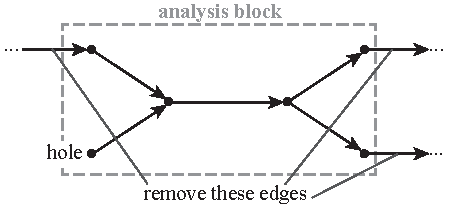
\includegraphics[width=3in]{images/analysis_block_hole}
		\end{center}
		\vspace{-20pt}
	\caption{Example variable node indicating a hole.}
	\label{f:hole}
	\end{figure}

	\item The second step is to detect collisions and to then disconnect enough connection edges so that the collisions are resolved. The set of variable nodes which contain collisions is created as
	\begin{equation}
	S_\txt{nodes} = \{v \in V_M \st t_\txt{node}(v) = \txt{`variable'} \txt{ and } \txt{deg}^-(v) > \txt{deg}_u^-(v) \}.
	\end{equation}
	For each collision node we can construct a set contained the edges directed in. The set containing all of these sets is constructed as
	\begin{equation}
	S_\txt{edges} = \big \{ \{(x,y) \in E_M\} \st y \in S_\txt{nodes} \big \}
	\end{equation}
	Let $J=\{1,2,\ldots,|S_\txt{edges}|\}$ be an indexing set for $S_\txt{edges}$ such that each $S_{\txt{edges},j}$ corresponds to a set in $S_\txt{edges}$ for $j \in J$. 
	An example collision is shown in Fig.~\ref{f:collision} to indicate the definition of $S_{\txt{edges},j}$. 
	We can assume that $J$ also indexes $S_\txt{nodes}$ because there is a one--to--one correspondence between the elements in $S_\txt{nodes}$ and the elements in $S_\txt{edges}$ (which are sets). 
	Then we may construct sets of edges as
	\begin{equation}
	B_j = \big \{e_k \in S_{\txt{edges},j} \st k \in \{1,2,\ldots,K\} \txt{ with } K \leq \txt{deg}_u^-(v_j) \big \}, \ j \in J,
	\end{equation}
	which means that each set $B_j$ is constructed from the set $S_{\txt{edges},j}$ by taking only as many edges as are allowed by the upper in--degree limit of $v_j$. The construction of each $B_j$ corresponds to making a decision on which edges to include and which edges not to include. Then let
	\begin{equation}
	C_{F,2} = \{ e \in C_{F,1} \st e \in B_j \txt{ for some } j \in J\},
	\end{equation}
	\begin{equation}
	E_{F,2} = E_M \setminus (C_M \setminus C_{F,2})
	\end{equation}
	and
	\begin{equation}
	F_2 = (V_M,E_{F,2})
	\end{equation}
	\begin{figure}[htb!]
		\begin{center}
		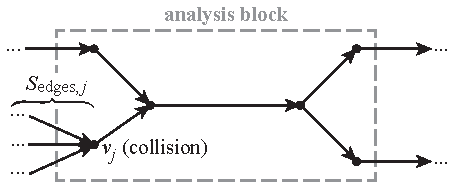
\includegraphics[width=3in]{images/analysis_block_collision}
		\end{center}
		\vspace{-20pt}
	\caption{Example variable node indicating a collision.}
	\label{f:collision}
	\end{figure}

	\item The third and final step is to remove any unused nodes and edges. The indexing set for only the analysis blocks with at least one used local output may be constructed as ((pruning))
	\begin{equation}
	I_F =  \{i \in I \ | \ \exists v \in V_{A_i} \txt{ such that }  t_\txt{node}(E_{F,2}^{-1}(v))=\txt{`model'} \txt{ and } \txt{deg}^+(v) > 0 \},
	\end{equation}
	where the degree is calculated with respect to $F_2$. This set excludes both the analysis blocks that were unused in the original MCG and those that became unused in step 1 or step 2.

	The set of used global inputs is constructed as
	\begin{equation}
	V_{\txt{in},F} = \Big\{v \in V_\txt{in} \ \Big| \ |\{(x,y) \in E_{F,2}(v) \st y \in V_{A_i} \txt{ for } i \in I_F  \}| > 1 \Big\},
	\end{equation}
	which requires that at least two edges directed out of the nodes in $V_{\txt{in},F}$ must be to the analysis blocks indexed by $I_F$.

	Finally, the set of nodes and edges describing a fundamental problem formulation is given by
	\begin{equation}
	V_F = V_{\txt{in},F} \cup V_\txt{out} \cup \left( \bigcup_{i \in I_F} V_{A_i} \right),
	\end{equation}
	\begin{equation}
	C_{F} = \{ (x,y) \in C_{F,2} \st x,y \in V_F\},
	\end{equation}
	\begin{equation}
	E_F = C_F \cup \left( \bigcup_{i \in I_F} E_{A_i} \right),
	\end{equation}
	\begin{equation}
	F = (V_F,E_F).
	\end{equation}

	\end{enumerate}
